\documentclass[12pt]{article}
\usepackage[left=1cm, right=1cm, top=2cm,bottom=1.5cm]{geometry} 

\usepackage[parfill]{parskip}
\usepackage[utf8]{inputenc}
\usepackage[T2A]{fontenc}
\usepackage[russian]{babel}
\usepackage{enumitem}
\usepackage[normalem]{ulem}
\usepackage{amsfonts, amsmath, amsthm, amssymb, mathtools}
\usepackage{tabularx}
\usepackage{hhline}

\usepackage{accents}
\usepackage{fancyhdr}
\pagestyle{fancy}
\renewcommand{\headrulewidth}{1.5pt}
\renewcommand{\footrulewidth}{1pt}

\usepackage{graphicx}
\usepackage[figurename=Рис.]{caption}
\usepackage{subcaption}
\usepackage{float}

%%Наименование папки откуда забирать изображения
\graphicspath{ {./images/} }

%%Изменение формата для ввода доказательства
\renewcommand{\proofname}{$\square$  \nopunct}
\renewcommand\qedsymbol{$\blacksquare$}

%%Изменение отступа на таблицах
\addto\captionsrussian{%
	\renewcommand{\proofname}{$\square$ \nopunct}%
}
%% Римские цифры
\newcommand{\RN}[1]{%
	\textup{\uppercase\expandafter{\romannumeral#1}}%
}

%% Для удобства записи
\newcommand{\MR}{\mathbb{R}}
\newcommand{\MQ}{\mathbb{Q}}
\newcommand{\MN}{\mathbb{N}}
\newcommand{\MI}{\mathrm{I}}
\newcommand{\MJ}{\mathrm{J}}
\newcommand{\MH}{\mathrm{H}}
\newcommand{\MT}{\mathrm{T}}
\newcommand{\MU}{\mathcal{U}}
\newcommand{\MV}{\mathcal{V}}
\newcommand{\VN}{\varnothing}
\newcommand{\VE}{\varepsilon}

\theoremstyle{definition}
\newtheorem{defn}{Опр:}
\newtheorem{rem}{Rm:}
\newtheorem{prop}{Утв.}
\newtheorem{exrc}{Упр.}
\newtheorem{lemma}{Лемма}
\newtheorem{theorem}{Теорема}
\newtheorem{corollary}{Следствие}

\newenvironment{cusdefn}[1]
{\renewcommand\thedefn{#1}\defn}
{\enddefn}

\DeclareRobustCommand{\divby}{%
	\mathrel{\text{\vbox{\baselineskip.65ex\lineskiplimit0pt\hbox{.}\hbox{.}\hbox{.}}}}%
}
%Короткий минус
\DeclareMathSymbol{\SMN}{\mathbin}{AMSa}{"39}
%Длинная шапка
\newcommand{\overbar}[1]{\mkern 1.5mu\overline{\mkern-1.5mu#1\mkern-1.5mu}\mkern 1.5mu}
%Функция знака
\DeclareMathOperator{\sgn}{sgn}

%Обозначение константы
\DeclareMathOperator{\const}{\text{const}}

%Интеграл в большом формате
\DeclareMathOperator{\dint}{\displaystyle\int}

\newcommand{\smallerrel}[1]{\mathrel{\mathpalette\smallerrelaux{#1}}}
\newcommand{\smallerrelaux}[2]{\raisebox{.1ex}{\scalebox{.75}{$#1#2$}}}

\newcommand{\smallin}{\smallerrel{\in}}
\newcommand{\smallnotin}{\smallerrel{\notin}}

\newcommand*{\medcap}{\mathbin{\scalebox{1.25}{\ensuremath{\cap}}}}%
\newcommand*{\medcup}{\mathbin{\scalebox{1.25}{\ensuremath{\cup}}}}%

\makeatletter
\newcommand{\vast}{\bBigg@{3.5}}
\newcommand{\Vast}{\bBigg@{5}}
\makeatother

%Скалярное произведение
\DeclarePairedDelimiterX{\inner}[2]{\langle}{\rangle}{#1, #2}

%Подпись символов снизу
\newcommand{\ubar}[1]{\underaccent{\bar}{#1}}

\begin{document}
\lhead{Математический анализ - \RN{2}}
\chead{Шапошников С.В.}
\rhead{Лекция - 16}
\section*{Теорема о неявной функции}
\subsection*{Множество уровня гладких функций}
Рассмотрим функцию $F\colon \MR^2 \to \MR, F(x,y)$. В прошлый раз мы задались вопросом: любое ли множество может являться множеством уровня:
$$
	\{(x,y)\colon F(x,y) = \const\}
$$
Мы успели понять следующие моменты:
\begin{enumerate}[label ={\arabic*)}]
	\item Если $F$ - произвольная, то любое множество может быть множеством уровня. Например:
	$$
		F(x,y) = \MI_A =  
		\begin{cases}
			1, & (x,y) \in A \\
			0, & \text{иначе}
		\end{cases} \Rightarrow A = \{(x,y)\colon F(x,y) = 1 \}
	$$
	\item Если $F$ - непрерывна, тогда множество уровня - замкнутое множество. Этот факт верен в любом метрическом пространстве.
	\begin{proof}
		Пусть $(X,\rho)$ - метрическое пространство, $F \colon X \to \MR$ - непрерывна. Рассмотрим множество: 
		$$
			A = \{ x \mid F(x) = c \}
		$$ 
		и возьмем последовательность точек $x_n$ которая сходится к $x_0$. По непрерывности будет верно:
		$$
			x_n \to x_0 \Rightarrow f(x_n) \to f(x_0), \, \forall n, \, f(x_n) = c \Rightarrow f(x_0) = \lim\limits_{n \to \infty} f(x_n) = c
		$$
		Тем самым, вместе с любой сходящейся последовательностью это множество содержит и её предел, следовательно множество замкнуто.
	\end{proof}
\end{enumerate}
Здесь сразу же возникает вопрос, а всякое ли замкнутое множество является множеством уровня?
\begin{prop}
	В метрическом пространстве $(X, \rho)$ для всякого замкнутого множества $A$ существует непрерывная функция $F \colon X \to \MR$ такая, что:
	$$
		\{x \mid F(x) = 0 \} = A
	$$
\end{prop}
\begin{proof}
	Рассмотрим следующую функцию:
	$$
		F(x) = \text{dist}(x,A) = \inf\limits_{y \in A}\rho(x,y)
	$$
	Пусть $F(x) = 0$ тогда: 
	$$
		\inf\limits_{y \in A}\rho(x,y) = 0 \Rightarrow \forall B(x,r), \, \exists \, y \in B(x,r) \cap A
	$$ 
	Если $x \notin A$, то $x$ - граничная точка (поскольку тогда в шаре лежат как точки $\in A$, так и точки $\notin A$), но граничные точки принадлежат $A$, поскольку $A$ замкнуто $\Rightarrow x \in A$. 
	
	Почему функция непрерывная? Рассмотрим разность значений функции в точках $x_1$ и $x_2$:
	$$
		F(x_1) - F(x_2) = \inf\limits_{y \in A}\rho(x_1,y) - \inf\limits_{y \in A}\rho(x_2,y)
	$$
	Возьмем $y$ такой, что:
	$$
		\forall \VE > 0,\, \exists \, y_\VE \colon \inf\limits_{y \in A}\rho(x_2,y) > \rho(x_2,y_\VE) - \VE
	$$
	Тогда оценим разность значений функции в точках $x_1$ и $x_2$ сверху:
	$$
		\inf\limits_{y \in A}\rho(x_1,y) - \inf\limits_{y \in A}\rho(x_2,y) \leq \rho(x_1, y_\VE) - \rho(x_2, y_\VE) + \VE \leq \rho(x_1, x_2) + \VE
	$$
	Устремляя $\VE$ к нулю, мы получим, что: 
	$$
		F(x_1) - F(x_2) \leq \rho(x_1,x_2) \Rightarrow |F(x_1) - F(x_2)| \leq \rho(x_1,x_2)
	$$
	где последнее неравенство верно в силу произвольности $x_1, x_2$.
\end{proof}
\begin{prop}
	Пусть $A$ - замкнутое подмножество $\MR^n$. Тогда существует непрерывно дифференцируемая функция $f \colon \MR^n \to \MR$ такая, что:
	$$
		A = \{ x \mid f(x) = 0  \}
	$$
\end{prop}
Данное утверждение достаточно трудоемко, поэтому приведем только идею для доказательства.

\textbf{\uline{Идея доказательства}}: Пусть $n = 2$ для наглядности. Поскольку $A$ замкнуто, то его дополнение - открыто. Мы знаем, что открытое множество состоит из открытых шаров, а поскольку мы можем выбирать шары $B_j$ рационального радиуса с центром в рациональной точке, то их будет счетное множество и тогда дополнение к замкнутому множеству будет следующим:
$$
	\MR^2 \setminus A = \bigcup\limits_j B_j
$$
Далее, построим такие функции, что их значения будут зануляться на границах этих шаров (в плоскости на границах круга), а внутри это будет строго положительная функция. 

Например, такую функцию можно построить на основе $e^{-\tfrac{1}{1 - x^2}}$ на отрезке $[-1,1]$. Тогда на единичном круге аналогичная функция будет иметь вид: $e^{-\tfrac{1}{1 - r^2}}$. Теперь сдвигая и масштабируя её, можем построить такую функцию на любом шаре $\Rightarrow \forall B_j, \, \exists \, \psi_j$. Пусть $|\psi_j| < \tfrac{1}{2^j}$ и $|\psi_j^\prime| < \tfrac{1}{2^j}$.

Искомая функция: 
$$
	F(x) = \displaystyle\sum\limits_{j=1}^{\infty}\psi_j(x)
$$ 
Тогда если взять любую точку не из $A$, то хотя бы одна из функций в ряду окажется строго положительной $\Rightarrow F(x) = 0 \Leftrightarrow x \in A$. Функция непрерывная, поскольку ряд сходится равномерно по признаку Вейрштрасса и равномерный предел непрерывных функций это непрерывная функция.

Если мы продифференцируем этот ряд по одной переменной, то получим следующий ряд:
$$
	\dfrac{\partial F(x)}{\partial x_k} = \displaystyle\sum\limits_{j=1}^{\infty}\dfrac{\partial}{\partial x_k}\psi_j(x)
$$
Этот ряд будет равномерно сходится по построению (производные ограничены сверху), исходный ряд также сходится равномерно, тогда предельная функция дифференцируема и её производная это предел производных.

\newpage
\subsection*{Теорема о неявной функции в $\MR^2$}
Пусть есть функция $F\colon \MR^2 \to \MR$. Хотим узнать как устроено множество уровня у функции $F$:
$$
	\{(x,y)\colon F(x,y) = 0\}
$$
Как обсудили ранее, это может быть почти любое множество, но в большинстве примеров это какие-то линии. Теорема о неявной функции говорит в каком случае мы будем видеть в качестве таких $(x,y)$ просто набор линий (графиков функций) на плоскости.

\begin{theorem}\textbf{(О неявной функции для $\MR^2$)} 
	Пусть $F$ непрерывно дифференцируема в окрестности точки $(x_0, y_0)$. Если выполнены следующие условия:
	\begin{enumerate}[label ={\arabic*)}]
		\item $F(x_0,y_0) = 0$;
		\item $\tfrac{\partial F}{\partial y}(x_0,y_0) \neq 0$;
	\end{enumerate}
	то $\exists \, \MU(x_0),\, \MV(y_0)$ - открытые множества и $f \colon \MU(x_0) \to \MV(y_0)$ - непрерывно дифференцируемая функция такие, что: 
	$$
		\forall (x,y) \in \MU \times \MV, \, F(x,y) = 0 \Leftrightarrow y = f(x)
	$$
\end{theorem}
\textbf{\uwave{Геометрический смысл}}: Мы хотим узнать, как устроено множество точек $\{(x,y)\colon F(x,y) = 0\}$ локально в окрестности точки $(x_0,y_0)$. Утверждается что найдется прямоугольник $\MU \times \MV$ такой, что в нём будет просто график функции $y = f(x)$.
\begin{figure}[H]
	\centering
	\includegraphics[width=0.35\textwidth]{16_1.eps}
	\caption{Смысл теоремы о неявной функции.}
	\label{16_1}
\end{figure}
Само множество при этом может быть достаточно сложно устроено, но взяв некоторую точку и рассмотрев окрестность вокруг неё, мы увидим график функции. Следовательно, картинка целиком будет составлена из таких локальных функций.
\begin{figure}[H]
	\centering
	
\includegraphics[width=0.25\textwidth]{16_2.eps}
	\caption{Локальное увеличение множества уровня.}
	\label{16_2}
\end{figure}
\begin{rem}
	В теореме ситуация будет симметричной, если потребовать $\tfrac{\partial F}{\partial x}(x_0,y_0) \neq 0$. И тогда $x = g(y)$. В любом случае, если $\nabla F\neq 0$, то локально мы будем наблюдать график функции.
\end{rem}
\textbf{\uwave{Алгебраический смысл}}: Есть уравнение $F(x,y) = 0 \Rightarrow$ хотим найти чему будет равен $y$ (то есть решить уравнение). Теорема говорит о том, что должно быть выполнено, чтобы мы могли это сделать:
\begin{enumerate}[label ={\arabic*)}]
	\item Бессмысленно искать решения там, где их нет $\Rightarrow$ хотя бы в одной точке должно выполнятся это равенство: $F(x_0,y_0) = 0$;
	\item Должна быть зависимость функции $F$ от $y$ или если по-другому: $\tfrac{\partial F}{\partial y}(x_0,y_0) \neq 0$;
\end{enumerate}
По теореме, если эти два условия выполнены, то существует теоретическая возможность решить уравнение и найти $y = f(x)$.
\begin{proof}
	Сделаем замену координат:
	$$
		\Psi \colon \left\{
		\begin{array}{lcl}
			u& = &x \\
			v& = &F(x,y)
		\end{array}\right.
	$$
	Тогда точка $(x_0,y_0)$ перейдет в точку $(x_0, F(x_0,y_0)) = (x_0,0)$. 
	\begin{figure}[H]
		\centering
		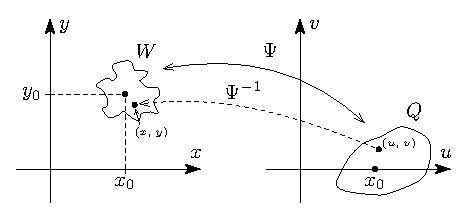
\includegraphics[width=0.55\textwidth]{16_3.eps}
		\caption{Замена координат в теореме о неявной функции.}
		\label{16_3}
	\end{figure}
	Чтобы быть уверенным, что это есть замена координат (т.е. можно было перевести одни в другие и вернуться обратно) по теореме об обратной функции необходимо рассмотреть матрицу Якоби:
	$$	
		J_{\Psi} = 
		\begin{pmatrix}
			\tfrac{\partial u}{\partial x} & \tfrac{\partial u}{\partial y}\\
			\tfrac{\partial v}{\partial x} & \tfrac{\partial v}{\partial y}
		\end{pmatrix} =
		\begin{pmatrix}
			1 & 0 \\
			\tfrac{\partial F}{\partial x} & \tfrac{\partial F}{\partial y}
		\end{pmatrix}
		\Rightarrow \det{\big(J_\Psi(x_0,y_0)\big)} = \tfrac{\partial F}{\partial y}(x_0,y_0) \neq 0
	$$
	Определитель этой матрицы в точке $(x_0,y_0)$ не ноль $\Rightarrow$ она обратима $\Rightarrow$ выполняются условия теоремы об обратной функции. Тогда найдутся окрестность $W$ точки $(x_0, y_0)$ и окрестность $Q$ точки $(x_0, 0)$ такие, что функция $\Psi \colon W \to Q$ - диффеоморфизм между ними. В том числе, есть обратное отображение:
	$$
		\Psi^{-1} \colon \left\{
		\begin{array}{lcl}
			x& = &u \\
			y& = &g(u,v)
		\end{array}\right.
	$$
	По той же теореме $\Psi^{-1}$ и в частности $g$ - непрерывно дифференцируемы. Поскольку окрестность $W$ произвольная и точка $(x_0, y_0)$ - внутренняя, то выберем интервалы $B(x_0) \subset W$ и $B(y_0) \subset W$ такими, что получим прямоугольник внутри $W$: 
	$$
		B(x_0), B(y_0) \subset W \colon B(x_0)\times B(y_0) \subset W
	$$
	\begin{figure}[H]
		\centering
		\includegraphics[width=0.55\textwidth]{16_4.eps}
		\caption{Выделение прямоугольника $B(x_0)\times B(y_0)$ внутри множества $W$.}
		\label{16_4}
	\end{figure}
	Рассмотрим образ этого прямоугольника: $\Psi\big(B(x_0)\times B(y_0)\big) \subset Q$.
	Очевидно, что это будет множество содержащее точку $(x_0,0)$, а поскольку неизвестно лежит ли точка из множества $F(x,y) = 0$ над каждой точкой из $B(x_0)$ , то рассмотрим образ прямоугольника в пересечении с осью $Ou$:
	$$
		\Psi\big(B(x_0)\times B(y_0)\big) \cap \{(u,v) \colon v = 0 \, \} = \MU(x_0)
	$$
	Полученное множество обозначим как $\MU(x_0)$. Мы берем пересечение, поскольку нам необходимо, чтобы над каждой точкой $x \in \MU(x_0)$ был график функции. Само по себе $B(x_0)$ не подходит, поскольку возможно отсутствие графика над частью этого множества. Заметим также, что $\MU(x_0)$ - открытое множество, поскольку пересечение открытого множества с осью - открыто.
	\begin{rem}
		Конечно можно взять множество $B(x_0)$ но придется брать его малым интервалом, чтобы над ним был график функции.
	\end{rem}
	\begin{figure}[H]
		\centering
		\includegraphics[width=0.55\textwidth]{16_5.eps}
		\caption{Построение множества $\MU(x_0)$.}
		\label{16_5}
	\end{figure}
	В качестве $\MV(y_0)$ возьмем интервал $B(y_0) \Rightarrow \MV(y_0) = B(y_0)$. Рассмотрим образ $\Psi$ следующего множества:
	$$
		\Psi\big(\{(x,y) \mid x \in \MU(x_0), \, y \in \MV(y_0), \, F(x,y) = 0 \}\big) = \{(u,v) \mid u \in \MU(x_0), \, v = 0 \}
	$$
	Проверим, что это действительно так:
	\begin{proof}\hfill\\
		$(\Rightarrow)$ Под действием отображения $\Psi$ верно $u =x, \, v = F(x,y) \Rightarrow x \in \MU(x_0) \Rightarrow u \in \MU(x_0)$, $v = F(x,y) = 0$.
		
		$(\Leftarrow)$ По определению множества $\MU(x_0)$, мы взяли пересечение образа прямоугольника с прямой $v = 0$. Тогда каждая точка из $\MU(x_0)$, в частности, есть образ какой-то точки из прямоугольника $B(x_0) \times B(y_0)$. Получается, что $\forall (u,v), \, \exists \, (x,y) \colon u = x, \, v = F(x,y)$, но $v = 0$ и $u \in \MU(x_0) \Rightarrow x \in \MU(x_0), \, F(x,y) = 0$.
	\end{proof}
	\begin{figure}[H]
		\centering
		\includegraphics[width=0.55\textwidth]{16_6.eps}
		\caption{Отображение $\{(x,y) \mid x \in \MU(x_0), \, y \in \MV(y_0)\}$ в $\Psi\big(\{(x,y) \mid x \in \MU(x_0), \, y \in \MV(y_0)\}\big)$ и обратно.}
		\label{16_6}
	\end{figure}
	Тогда будет верно следующее:
	$$
		(x,y) \in \MU(x_0) \times \MV(y_0) \colon F(x,y) = 0 \overset{\Psi}{\Leftrightarrow}
		\left\{\begin{array}{l}
			x = u \in \MU(x_0) \\
			v = F(x,y) = 0
		\end{array}\right. 
	 	\overset{\Psi^{-1}}{\Leftrightarrow}
		\left\{\begin{array}{l}
	 		x = u \in \MU(x_0) \\
	 		y = g(u,v), \, v = 0
	 	\end{array}\right. 
	$$
	где последнее выражение означает следующее:
	$$
		\left\{\begin{array}{l}
			x = u \in \MU(x_0) \\
			y = g(u,v), \, v = 0
		\end{array}\right. 
		\Leftrightarrow y = g(x,0), \, x \in \MU(x_0)
	$$
	То есть в качестве функции $f(x)$ возьмем функцию $g(x,0)$ и получаем, что в квадрате $B(x_0)\times B(y_0)$ множество уровня $F(x,y) = 0$ это в точности график функции $f(x)$ над $\MU(x_0)$. Итого:
	$$
		(x,y) \in \MU \times \MV \colon F(x,y) = 0 \Leftrightarrow y = g(x,0) = f(x), \, x \in \MU(x_0)
	$$
	Более того, полученная функция $f(x)$ непрерывно дифференцируема по теореме об обратной функции.
\end{proof}

\begin{rem}
	Функция $F$ из теоремы в новых координатах $u$ и $v$ имеет вид: 
	$$
		\left\{\begin{array}{l}
			x(u,v) = u \\
			y(u,v) = g(u,v)
		\end{array}\right.
		\Rightarrow \widetilde{F}(u,v) = F\big(x(u,v),y(u,v)\big) = F\big(u, g(u,v) \big) = v
	$$ 
	где последнее равенство справедливо в силу замены $v = F(x,y)$. Рассмотрим это  подробнее.
	
	Пусть $\exists$ плоскость и над ней $\exists$ какая-то функция $F \colon \forall$ точки $A$ в этой плоскости мы знаем $F(A)$. Затем, мы захотели увидеть какую-то формулу и ввели систему координат $Oxy$.
	\begin{figure}[H]
		\centering
		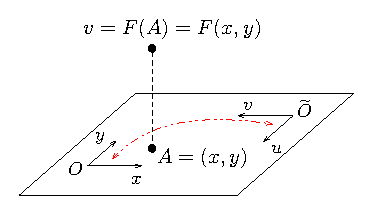
\includegraphics[width=0.35\textwidth]{16_7.eps}
		\caption{Введение систем координат на плоскости для функции $F$.}
		\label{16_7}
	\end{figure}
	Тогда $A$ стала точкой с координатами $(x,y)$ и вместо $F(A)$ теперь пишем $F(x,y)$. Затем по теореме о неявной функции, если верно что $\tfrac{\partial F}{\partial y} \neq 0$, то можно ввести другую систему координат $\widetilde{O} uv$, таким образом, что: 
	$$
		 F(x,y) = F(A) = v
	$$
	то есть точке $A$ будет сопоставляться вторая координата.
	
	\textbf{\uline{Итог}}: По крайней мере локально, в удобной системе координат, функция из теоремы о неявной функции это просто координата.
\end{rem}
\begin{rem}
	Заметим также, что в теореме есть условие $F(x_0,y_0) = 0$. Возьмем любую функцию двух переменных $F(x,y)$, но такую, что $\tfrac{\partial F}{\partial y} \neq 0$ и рассмотрим функцию:
	$$
		G(x,y) = F(x,y) - F(x_0,y_0)
	$$
	У неё $\tfrac{\partial G}{\partial y} \neq 0$ и в точке $(x_0,y_0)$ она очевидно равна нулю: $G(x_0,y_0) = 0$. Тогда можно ввести систему координат так, что в новых координатах это $v$:
	$$
		G(x,y) = F(x,y) - F(x_0,y_0) = v
	$$
	Поскольку для $x$ и $y$ ситуация симметричная, то всегда изначально их можно поменять местами в системе координат и тогда вместо  $\tfrac{\partial F}{\partial y} \neq 0$ будет $\tfrac{\partial F}{\partial x} \neq 0$. Таким образом, если:
	$$
		\nabla F = (\tfrac{\partial F}{\partial x}, \tfrac{\partial F}{\partial y}) \neq 0
	$$ 
	то локально можно ввести такую систему координат, что эта функция в новых координатах $\widetilde{O} uv$ будет иметь следующий вид:
	$$
		\widetilde{F}(u,v) = c + v, \, c \in \MR
	$$
	\textbf{\uline{Итог}}: Если у функции градиент невырожденный, то она локально является линейной (координатно линейная) плюс константа. Если не видим линейных функций, то это проблема с системой координат $\Rightarrow$ выберете правильную систему координат и работайте с обычной линейной функцией.
\end{rem}
\begin{rem}
	Одновременно с этим, нужно заметить, что переход из системы координат $Oxy$ в $\widetilde{O} uv$ может быть очень сложным и обычно на практике это редко работает. Поэтому если нужно узнать что-то в старых координатах, то данное утверждение помогает только теоретически.
\end{rem}
\begin{rem}
	Линии уровня у функции $\widetilde{F}(u,v) = c + v$ это $c + v = \const$ (или по-другому $v = \const$), то есть это просто горизонтальные прямые. 
	
	Таким образом, линии уровня у функций с невырожденным градиентом локально в правильной системе координат это просто прямые, а обратное отображение эти прямые превращает в графики функций. Ровно про это и говорит теорема о неявной функции.
\end{rem}

\newpage
\subsection*{Теорема о неявных функциях}
\begin{theorem}\textbf{(О неявной функции в общем виде)} 
	Пусть $F \colon \MR_x^n \times \MR_y^m \to \MR^m$ непрерывно дифференцируема в окрестности точки $(x_0, y_0)$. Если выполнены следующие условия:
	\begin{enumerate}[label ={\arabic*)}]
		\item $F(x_0,y_0) = 0$;
		\item $\det{\big(\tfrac{\partial F_i}{\partial y_j}(x_0,y_0)\big)} \neq 0$;
	\end{enumerate}
	то $\exists \, \MU(x_0),\, \MV(y_0)$ - открытые множества и $f \colon \MU(x_0) \to \MV(y_0)$ - непрерывно дифференцируемая функция такие, что: 
	$$
		\forall (x,y) \in \MU \times \MV, \, F(x,y) = 0 \Leftrightarrow y = f(x)
	$$
\end{theorem}
\textbf{\uwave{Алгебраический смысл}}: Также, как и раньше мы хотим решить систему уравнений. Распишем каждый из элементов покомпонентно:
$$
	F = \begin{pmatrix}
		F_1 \\
		\vdots \\
		F_m
	\end{pmatrix}, \, 
	x = \begin{pmatrix}
		x_1 \\ 
		\vdots \\
		x_n
	\end{pmatrix}, \,
	y = \begin{pmatrix}
		y_1 \\
		\vdots \\
		y_m
	\end{pmatrix}, \, 
	(x,y) \to \begin{pmatrix}
		F_1(x,y) \\
		\vdots \\
		F_m(x,y)
	\end{pmatrix},\,
	\left\{
	\begin{array}{ccc}
		F_1(x_1, \dotsc, x_n, y_1, \dotsc, y_m) & = &  0 \\
		\vdots & \ddots & \vdots \\
		F_m(x_1, \dotsc, x_n, y_1, \dotsc, y_m) & = &  0 
	\end{array}
	\right.
$$
Решить данную систему это тоже самое, что и $y_j$ выразить как функции от $x_1, \dotsc, x_n$:
$$
	y_j = y_j(x_1, \dotsc, x_n), \, \forall j = \overline{1,m}
$$
Как мы знаем, системы линейных уравнений из $m$ уравнений решаются, когда есть $m$ неизвестных. В данном случае переменные $x$ выступают как параметры или свободные неизвестные, а $y$ как главные неизвестные. Этим можно объяснить размерность: у нас $m$ неизвестных $y \Rightarrow m$ уравнений.

Линейные системы однозначно решаются, когда их матрицы невырождены. В данном случае, матрица Якоби это линейная часть этой системы из функций. Мы знаем что дифференцируемые отображения локально похожи на аффинные (или линейные) $\Rightarrow$ по теореме, если матрица линейной части невырождена, то система должна решаться.

Аналогично двумерному случаю, теорема о неявных функциях это теорема о том, когда можно решить систему уравнений:
\begin{enumerate}[label ={\arabic*)}]
	\item Когда есть хотя бы одно решение: $F(x_0,y_0) = 0$;
	\item Матрица Якоби должна быть невырожденной в нём: $\det{\big(\tfrac{\partial F_i}{\partial y_j}(x_0,y_0)\big)} \neq 0$;
\end{enumerate}

\textbf{Пример}: Рассмотрим следующую систему:
$$
	\left\{\begin{array}{ccc}
		F_1(x_1, y_1, y_2) & = &  0 \\
		F_2(x_1, y_1, y_2) & = &  0 
	\end{array}\right.
$$
Нужно найти $y_1, y_2$, переменную $x_1$ воспринимаем как параметр. Пусть мы не знаем теорему о неявных функциях. Каким образом будем искать решение? Например так:
$$
	\left\{
	\renewcommand\arraystretch{1.3}
		\begin{array}{c}
				F_1(x_1, y_1,y_2) \approx F_1(x_1,y_1^0, y_2^0) + \tfrac{\partial F_1}{\partial y_1}{\cdot}(y_1 - y_1^0) + \tfrac{\partial F_1}{\partial y_2}{\cdot}(y_2 - y_2^0)\\
				F_2(x_1, y_1,y_2) \approx F_2(x_1,y_1^0, y_2^0) + \tfrac{\partial F_2}{\partial y_1}{\cdot}(y_1 - y_1^0) + \tfrac{\partial F_2}{\partial y_2}{\cdot}(y_2 - y_2^0)
		\end{array}
	\right.
$$
и тогда исходная система уравнений превратится в линейную:
$$
	\left\{
	\renewcommand\arraystretch{1.3}
	\begin{array}{ccc}
		\tfrac{\partial F_1}{\partial y_1}{\cdot}y_1 + \tfrac{\partial F_1}{\partial y_2} {\cdot} y_2  & = &  C_1 \\
		\tfrac{\partial F_2}{\partial y_1}{\cdot}y_1 + \tfrac{\partial F_2}{\partial y_2} {\cdot} y_2  & = &  C_2
	\end{array}
	\right.
$$
Линейную систему уравнений можно решить, когда определитель её матрицы не равен нулю.

\textbf{\uline{Итог}}: нелинейные отбражения приближаются линейными $\Rightarrow$ для них решение системы уравнений находится исходя из теории алгебры, а теорема о неявных функциях говорит, что ровно такой же ответ будет верен для нелинейных отображений.

\textbf{\uwave{Геометрический смысл}}: Теорема утверждает, что если рассматривать множество:
$$
	\{(x,y) \in \MR_x^n \times \MR_y^m \mid F(x,y)= 0\}
$$
то локально, оно будет равносильно следующему:
$$
	\{(x,y) \in \MU(x_0) \times \MV(y_0) \mid y = f(x) \}
$$
что еще можно записать таким образом:
$$
	\big\{(x,y) \mid (x,y) = \big(x_1, \dotsc, x_n, f_1(x_1, \dotsc, x_n), \dotsc, f_m(x_1,\dotsc, x_n)\big), \, x = (x_1, \dotsc, x_n) \in \MU(x_0) \big\}
$$
То есть, множество $\{(x,y) \mid F(x,y)=0\}$ локально параметризуется переменными $(x_1, \dotsc, x_n)$. Следовательно, когда меняем $n$ параметров, то в $\MR_x^n \times \MR_y^m$ рисуется некая картинка.

\textbf{Пример}: Рассмотрим частный случай: $F \colon \MR_x^2 \times \MR_y^1 \to \MR$, это обычная функция трех переменных. Мы хотим понять что из себя представляет множество уровня $F(x_1, x_2, y) = 0$. Поскольку это функция трех переменных, то это множество в $\MR^3$ и по утверждению теоремы это $y = f(x_1, x_2)$.
\begin{figure}[H]
	\centering
	\includegraphics[width=0.3\textwidth]{16_8.eps}
	\caption{Введение систем координат на плоскости для функции $F$.}
	\label{16_8}
\end{figure}
Следовательно, мы получили \uwave{двумерную поверхность} $\big(x_1,x_2,f(x_1,x_2)\big)$, поскольку задаются $x_1, x_2$ и из них получается $f(x_1,x_2) \Rightarrow$ меняются два параметра и рисуется какое-то множество в $\MR^3$. 

Аналогично $\big(x_1, \dotsc, x_n, f_1(x_1, \dotsc, x_n), \dotsc, f_m(x_1,\dotsc, x_n)\big)$ задает \uwave{$n$-мерную поверхность}, то есть что нарисуем если будем менять $n$ параметров.

\textbf{\uline{Итог}}: множество решений системы:
$$
	\left\{
	\begin{array}{ccc}
		F_1(x_1, \dotsc, x_n, y_1, \dotsc, y_m) & = &  0 \\
		\vdots & \ddots & \vdots \\
		F_m(x_1, \dotsc, x_n, y_1, \dotsc, y_m) & = &  0 
	\end{array}
	\right.
$$
в координатах $x,y$ задает поверхность размерности $n$, то есть всё это множество можно запараметризовать первыми $n$ координатами: $(x_1, \dotsc, x_n)$. По аналогии с двумерным случаем, теорема утверждает что решение заданной системы это локально поверхность размерности $n$ (график функции).

Рассмотрим следующий пример системы уравнений:
$$
	\left\{
	\begin{array}{ccc}
		A_1(x - x_0) + B_1(y - y_0) + C_1(z - z_0)  & = &  0 \\
		A_2(x - x_0) + B_2(y - y_0) + C_2(z - z_0)  & = &  0
	\end{array}
	\right.
$$
В общем случае, одно уравнение задает плоскость (то есть двумерную поверхность), а два уравнения задают пересечение плоскостей $\Rightarrow$ задают кривую (то есть одномерную поверхность).

Например, была система из одного уравнения $F_1(x,y,z) = 0 \Rightarrow$ можно выразить $z = f(x,y)$ и получим двумерную поверхность. Если добавить еще одно уравнение $F_2(x,y,z) = 0$, то поверхности пересекутся и получится кривая в пространстве: $y = f(x), z = g(x)$. 

В многомерном случае, всего $n + m$ переменных, пересекли $m$ штук $\Rightarrow$ остался $n$-мерный объект (заменили все главные переменные через свободные).
\begin{proof}
	Практически полностью повторяет доказательство для $\MR^2$. Рассмотрим замену координат:
	$$
		\Psi \colon \left\{
		\begin{array}{ccc}
			u_1& = &x_1 \\
			\vdots & \ddots & \vdots \\
			u_n& = &x_n \\
			v_1& = &F_1(x,y) \\
			\vdots & \ddots & \vdots \\
			v_m& = &F_m(x,y)
		\end{array}\right. \Leftrightarrow  
		\left\{
		\begin{array}{lcl}
			u& = &x \\
			v& = &F(x,y)
		\end{array}\right.
	$$
	Рассмотрим матрицу Якоби данного отображения:
	$$
		J_\Psi =	
		\left(
		\renewcommand\arraystretch{1.2}
		\begin{array}{cccc|ccc}
			1 & 0 & \dotsc & 0 & 0 & \dotsc & 0 \\
			0 & 1 & \dotsc & 0 & 0 & \dotsc & 0 \\
			\vdots & \vdots & \ddots & \vdots & \vdots & \ddots & \vdots \\
			0 & 0 & \dotsc & 1 & 0 & \dotsc & 0  \\
			\hline
			* & * & \dotsc & * & \tfrac{\partial F_1}{\partial y_1} & \dotsc & \tfrac{\partial F_1}{\partial y_m} \\
			\vdots & \vdots & \ddots & \vdots & \vdots & \ddots & \vdots \\
			* & * & \dotsc & * & \tfrac{\partial F_m}{\partial y_1} & \dotsc & \tfrac{\partial F_m}{\partial y_m} 
		\end{array}
		\right)
	$$
	Определитель этой матрицы Якоби в точке $(x_0,y_0)$ будет равен $\det{\big(\tfrac{\partial F_i}{\partial y_j}(x_0,y_0)\big)} \neq 0$, как определитель блочно-диагональной матрицы $\Rightarrow$ эта матрица обратима и перед нами локальный диффеоморфизм. Тогда найдется окрестность $W$ точки $(x_0, y_0)$ и окрестность $Q$ точки $(x_0, 0)$ такие, что $\Psi \colon W \to Q$ это диффеоморфизм между ними. Более того, существует обратное отображение:
	$$
		\Psi^{-1} \colon 
		\left\{
		\begin{array}{lcl}
			x& = &u \\
			y& = &g(u,v)
		\end{array}
		\right.
	$$
	По той же теореме $\Psi^{-1}$ и в частности $g$ - непрерывно дифференцируемы. Поскольку окрестность $W$ произвольная и точка $(x_0, y_0)$ - внутренняя, то выберем открытые шары $B(x_0) \subset W$ и $B(y_0) \subset W$ такими, что получим прямоугольник внутри $W$: 
	$$
		B(x_0), B(y_0) \subset W \colon B(x_0)\times B(y_0) \subset W
	$$
	Рассмотрим образ этого прямоугольника: $\Psi\big(B(x_0)\times B(y_0)\big) \subset Q$.
	Очевидно, что это будет множество содержащее точку $(x_0,0)$, а поскольку неизвестно лежит ли точка из множества $F(x,y) = 0$ над каждой точкой из $B(x_0)$ , то рассмотрим образ прямоугольника в пересечении с осью $Ou$:
	$$
		\Psi\big(B(x_0)\times B(y_0)\big) \cap \{(u,v) \colon v = 0 \, \} = \MU(x_0)
	$$
	Полученное множество обозначим как $\MU(x_0)$. Мы берем пересечение, поскольку нам необходимо, чтобы над каждой точкой $x \in \MU(x_0)$ была поверхность. Само по себе $B(x_0)$ не подходит, поскольку возможно отсутствие поверхности над частью этого множества. Заметим также, что $\MU(x_0)$ - открытый шар, поскольку пересечение открытого множества с осями - открыто.

	В качестве $\MV(y_0)$ возьмем открытый шар $B(y_0) \Rightarrow \MV(y_0) = B(y_0)$. Рассмотрим образ $\Psi$ следующего множества:
	$$
		\Psi\big(\{(x,y) \mid x \in \MU(x_0), \, y \in \MV(y_0), \, F(x,y) = 0 \}\big) = \{(u,v) \mid u \in \MU(x_0), \, v = 0 \}
	$$
	Проверим, что это действительно так:
	\begin{proof}\hfill\\
		$(\Rightarrow)$ Под действием отображения $\Psi$ верно $u =x, \, v = F(x,y) \Rightarrow x \in \MU(x_0) \Rightarrow u \in \MU(x_0)$, $v = F(x,y) = 0$.
		
		$(\Leftarrow)$ По определению $\MU(x_0)$, мы взяли пересечение образа прямоугольника с гиперплоскостью $v = 0$. Тогда каждая точка из $\MU(x_0)$, в частности, есть образ какой-то точки из прямоугольника $B(x_0) \times B(y_0)$. Получается, что $\forall (u,v), \, \exists \, (x,y) \colon u = x, \, v = F(x,y)$, но $v = 0$ и $u \in \MU(x_0) \Rightarrow x \in \MU(x_0), \, F(x,y) = 0$.
	\end{proof}
	Тогда будет верно следующее:
	$$
		(x,y) \in \MU(x_0) \times \MV(y_0) \colon F(x,y) = 0 \overset{\Psi}{\Leftrightarrow}
		\left\{\begin{array}{l}
			x = u \in \MU(x_0) \\
			v = F(x,y) = 0
		\end{array}\right. 
		\overset{\Psi^{-1}}{\Leftrightarrow}
		\left\{\begin{array}{l}
			x = u \in \MU(x_0) \\
			y = g(u,v), \, v = 0
		\end{array}\right. 
	$$
	где последнее выражение означает следующее:
	$$
		\left\{\begin{array}{l}
			x = u \in \MU(x_0) \\
			y = g(u,v), \, v = 0
		\end{array}\right. 
		\Leftrightarrow y = g(x,0), \, x \in \MU(x_0)
	$$
	То есть в качестве функции $f(x)$ возьмем функцию $g(x,0)$ и получаем, что в квадрате $B(x_0)\times B(y_0)$ множество уровня $F(x,y) = 0$ это в точности поверхность $f(x)$ над $\MU(x_0)$. Итого:
	$$
		(x,y) \in \MU \times \MV \colon F(x,y) = 0 \Leftrightarrow y = g(x,0) = f(x), \, x \in \MU(x_0)
	$$
	и поверхность $f(x)$ непрерывно дифференцируема по теореме об обратной функции.
\end{proof}
\begin{rem}
	Пусть есть функция $f(x_1, \dotsc, x_n)$ и пусть $\tfrac{\partial f}{\partial x_n} \neq 0$, тогда  $\exists$ система координат $u_1, \dotsc, u_n$:
	$$
		f = \widetilde{f}(u_1, \dotsc, u_n) = \const + u_n
	$$
	То есть и в многомерном случае, если градиент функции $f$ не ноль, то локально её можно представить как константу плюс горизонтальную линию. Следовательно, множество уровня такой функции локально это $u_n = c$ (то есть это $(n-1)$-мерные гиперплоскости). 
\end{rem}

\end{document}